% ============================================================================
% RESULTS SECTION — draft 2026-09-02
%
% Figures live next to this file (paper_stuff/):
%   fig_results_01_replication.pdf  fig_results_02_nocue.pdf  fig_results_03_transfer.pdf
%   (regenerate with: python paper_stuff/make_results_figures.py — reads results/*.json only)
%
% Every number below traces to a checked-in artifact:
%   results/layer_sweep_full320-v3_{llama31_8b,llama31_70b,llama33_70b}.json   (Tables 1, 3; Figs 1, 3A)
%   results/nocue_sweep_full320-v3_*.json + provenance/full320-v3/nocue_sweep_run.json (Table 2; Fig 2)
%   results/full_layer_gap_erasure_summary.json                                 (integrated gap, rank-64; Fig 3B)
%   artifacts/format_bound_regrowth_bootstrap.json                              (min / final / widening CIs)
%   artifacts/full320_equal_n_llama31_8b_l12.json                               (appendix, tab:equaln)
%   artifacts/exploratory/full320_exact_logistic_estimator_reversal_conclusion_20260823/conclusion.json
%   results/surface_probes_v3_full320.json                                      (appendix, tab:text_controls, cue-excised rows)
%   paper_stuff/text_audit_full320_stated.json                                  (appendix, tab:text_controls, cue-present rows;
%        development-only run of paper_stuff/text_audit_full320.py — NOT yet a results/ artifact; rerun + check in)
%   results/v2/pilot80_sweep_full_llama3{1_8b,1_70b,3_70b}.json                 (appendix, tab:pilot; separate freeze)
%
% Packages assumed by this fragment: booktabs, graphicx, natbib (\citet), amsmath.
% Bib key devbunova2026format = Devbunova, arXiv:2603.19426 (as in plots/paper.tex).
%
% Wording rules kept from README/RULES: "stated response purpose", not "evaluation awareness";
% AUC and balanced accuracy (BA) reported separately; layers = one trajectory per checkpoint;
% projection results are frozen-activation diagnostics, not causal claims; 405B is unpinned/dev-only.
% ============================================================================

\section{Results}
\label{sec:results}

All probe results are reported for the three pinned checkpoints (Llama-3.1-8B,
Llama-3.1-70B, Llama-3.3-70B) at every transformer block. Where a single layer
is quoted it is the zero-based layer that maximizes the checkpoint's
decorrelated held-family-out AUC (8, 18 and 18; relative depths .26, .23 and
.23). This rule uses the decorrelated AUC only and was fixed before the no-cue
and projection analyses of Sections~\ref{sec:results_nocue}
and~\ref{sec:results_transfer} were run. Layers are treated as one depth
trajectory per checkpoint rather than as independent replicates, so every
pinned-layer number is shown with its trajectory
(Figures~\ref{fig:results_replication}--\ref{fig:results_transfer}).
Uncertainty intervals are 95\% percentile intervals from bootstraps over
complete payload blocks. AUC and balanced accuracy (BA, at the fitted zero
threshold) are reported separately throughout.

% ----------------------------------------------------------------------------
\subsection{The format trap replicates under content-matched control, and
decorrelated training recovers stated purpose}
\label{sec:results_replication}

\paragraph{Confounded training yields a format detector.}
A probe trained only on the naturally confounded diagonal (evaluation prompts
in benchmark format against deployment prompts in casual format) and evaluated
on all four cells separates the cells by format, not by purpose
(Table~\ref{tab:probe_comparison}, Figure~\ref{fig:results_replication}B).
At the selected layers its four-cell AUC is .600, .682 and .667 and its
balanced accuracy is .500, .528 and .508. Deployment prompts rendered in
benchmark format are called ``evaluation'' 100.0\%, 91.5\% and 97.4\% of the
time, and evaluation prompts in casual format are called ``deployment''
100.0\%, 98.0\% and 99.7\% of the time. The trap is not a property of the
selected layer: the deployment--benchmark false-positive rate never falls
below 91.5\% at any layer of any checkpoint, and confounded AUC stays between
.50 and .70 across depth (Figure~\ref{fig:results_replication}A). This
reproduces the central observation of \citet{devbunova2026format}, whose
standard probe classified 94.5\% of benchmark-formatted deployment prompts as
evaluation and 0\% of casual evaluation prompts as evaluation, here on a design
in which the same payload text appears in all four cells.

\paragraph{Decorrelated training recovers purpose.}
Training on all four cells, with format balanced against purpose, and testing
on a held-out purpose-vocabulary family gives AUC .989, .998 and .996 (BA
.941, .979 and .966). The decision is calibrated across cells: at Llama-3.1-8B,
93.0\% / 92.9\% of evaluation prompts are called evaluation in benchmark /
casual format and 4.3\% / 5.3\% of deployment prompts; the corresponding
figures are 97.9\% / 98.0\% and 2.2\% / 2.2\% at Llama-3.1-70B and 97.3\% /
96.9\% and 4.3\% / 3.5\% at Llama-3.3-70B. Every one of the 3,524 complete
minimal pairs is ordered correctly, with the evaluation member scoring above
its deployment twin. These numbers match the paired-probe row of
Devbunova's Table~2 (98.5\%, 100\%, 0\% and 7.2\% across her four cells), with
four differences in what the replication controls. Content is held fixed by
construction rather than matched by length, because each payload appears in
all four cells. Purpose is stated in the prompt rather than defined by the
source dataset. The test fold shares no purpose vocabulary with the training
folds, whereas her paired probe used an 80/20 random split of the pooled cells
(our folds do share payload blocks, so they test generalization to unseen
purpose wording, not to unseen tasks). And the result holds on three
checkpoints at every layer rather than on one checkpoint at selected layers.

\paragraph{Depth.}
Format is linearly decodable from the first block (format-probe AUC $\geq$
.999 at layer 0 in every checkpoint), whereas purpose emerges during the
forward computation: decorrelated AUC is .56, .65 and .65 at layer 0, crosses
.95 at layers 4, 7 and 7, peaks at 23--26\% relative depth, and declines
gradually to .913, .941 and .912 at the final layer
(Figure~\ref{fig:results_replication}A).

\begin{table}[ht]
\centering
\caption{
\textbf{Confounded probes follow format, while decorrelated probes recover
stated purpose.}
All results are reported at the zero-based layer maximizing each checkpoint's
decorrelated held-family-out AUC; relative depth is the layer index divided by
$L-1$. Confounded AUC and BA are evaluated over all four purpose-by-format
cells. DB$\rightarrow$eval is the percentage of deployment--benchmark prompts
classified as evaluation, and EC$\rightarrow$deploy the percentage of
evaluation--casual prompts classified as deployment; both are obtained by
converting positive probe scores to evaluation predictions and negative scores
to deployment predictions. BA is balanced accuracy at the same zero threshold.
}
\label{tab:probe_comparison}
\small
\setlength{\tabcolsep}{5pt}
\begin{tabular}{lccccc}
\toprule
Model
& \shortstack{Selected layer\\(relative depth)}
& \shortstack{Confounded\\AUC / BA}
& \shortstack{DB$\rightarrow$eval\\error (\%)}
& \shortstack{EC$\rightarrow$deploy\\error (\%)}
& \shortstack{Decorrelated\\AUC / BA} \\
\midrule
Llama-3.1-8B
& 8 (.26)
& .600 / .500
& 100.0
& 100.0
& .9888 / .941 \\

Llama-3.1-70B
& 18 (.23)
& .682 / .528
& 91.5
& 98.0
& .9984 / .979 \\

Llama-3.3-70B
& 18 (.23)
& .667 / .508
& 97.4
& 99.7
& .9959 / .966 \\
\bottomrule
\end{tabular}
\end{table}

\begin{figure}[t]
\centering
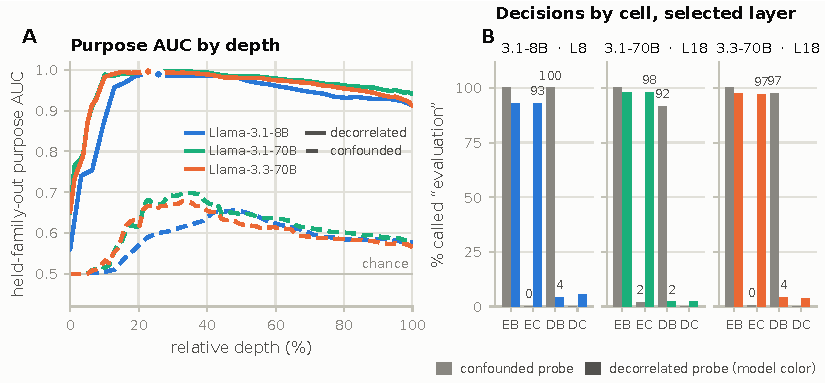
\includegraphics[width=\linewidth]{fig_results_01_replication.pdf}
\caption{
\textbf{Purpose decodability by depth, and the confound signature at the
selected layer.}
(A) Held-family-out purpose AUC of the decorrelated (solid) and confounded
(dashed) probes across relative depth for the three pinned checkpoints;
markers show the selected layers. Format is decodable from layer 0 (not
shown; AUC $\geq$ .999 everywhere), purpose forms by 10--20\% depth.
(B) Percentage of held-out prompts called ``evaluation'' in each
purpose-by-format cell at the selected layer, one panel per checkpoint, for
the confounded (gray) and decorrelated (colored) probes. Cells: EB
evaluation--benchmark, EC evaluation--casual, DB deployment--benchmark, DC
deployment--casual; the two off-diagonal cells are labeled. The confounded
probe answers by format; the decorrelated probe answers by purpose in both
formats.
}
\label{fig:results_replication}
\end{figure}

% ----------------------------------------------------------------------------
\subsection{The no-cue stratum: what format alone does to each probe}
\label{sec:results_nocue}

The 3,840 no-cue rows are the same payloads under the same 13 templates with
the purpose statement absent (2,080 benchmark, 1,760 casual). They carry no
purpose label, are never used for training, and belong to no vocabulary fold,
so each is scored by all five held-fold models and the scores are averaged.
For a probe with decision score $s$ we report the format shift
$\Delta = (\bar{s}_{\mathrm{bench}} - \bar{s}_{\mathrm{casual}}) /
\mathrm{SD}(s)$, where the SD is taken over the no-cue projections themselves,
with a cluster bootstrap over payload blocks (2,000 draws); the same contrast
taken within payload block agrees to within .01. In this unit a score that is
a pure two-point function of format saturates at 2.01 for this
benchmark/casual split. We also report the percentage of no-cue items that
fall on the ``evaluation'' side of the zero threshold, and the AUC with which
the purpose score alone ranks benchmark above casual items.

\paragraph{The confounded probe is a format detector on items that state no purpose.}
At every layer of every checkpoint the confounded probe calls essentially all
no-cue benchmark items ``evaluation'' and all no-cue casual items
``deployment'' (100.0\% / 0.0\% at the selected layers;
Table~\ref{tab:nocue}). Its shift is $+1.95$, $+1.93$ and $+1.93$, within 4\%
of the two-point ceiling, and its score ranks benchmark above casual with AUC
1.000 (Figure~\ref{fig:results_nocue}).

\paragraph{The decorrelated probe keeps a small, scale-dependent format residual.}
The repaired probe is not format-blind. At Llama-3.1-8B the shift at the
selected layer is $-0.13$ [$-0.19$, $-0.08$]: small, and in the direction of
``deployment'' for benchmark formatting. At the two 70B checkpoints it is
$+0.82$ [$+0.78$, $+0.86$] and $+0.70$ [$+0.65$, $+0.74$]: benchmark formatting
alone moves a purpose-free item toward ``evaluation'', and the purpose score
ranks no-cue benchmark above casual items with AUC .73 and .70 (.47 at 8B).
At the zero threshold the 70B probes call 27.6\% and 22.4\% of no-cue
benchmark items ``evaluation'' against 8.7\% and 4.1\% of casual items (2.5\%
and 7.2\% at 8B). The residual is depth-dependent
(Figure~\ref{fig:results_nocue}A): the 8B value at the selected layer is the
minimum of its trajectory and the 70B values lie near their maxima, and
averaged over all layers at which purpose is formed (decorrelated AUC $\geq$
.95) the shifts are $+0.23$, $+0.41$ and $+0.49$. The residual is also small
relative to the purpose signal itself: expressed against the stated
evaluation-minus-deployment score gap at the same layer it is $-2\%$, $+11\%$
and $+10\%$. The unpinned Llama-3.1-405B extension (NDIF deployment,
development evidence only) shows the same pattern, $+0.59$ [$+0.54$, $+0.64$]
at its selected layer with format AUC .67.

\paragraph{Relation to the 7.2\% residual.}
Devbunova's paired probe still called 7.2\% of benchmark-formatted deployment
prompts ``evaluation''. That number is a threshold rate on rewritten ShareGPT
queries, so it folds together format, source and rewriter differences, and it
cannot be read as a magnitude. The no-cue stratum isolates the format term:
identical payloads, identical templates, purpose absent, and a threshold-free
contrast with a block-bootstrap interval. On this measure decorrelated
training removes the trap (from about 2 to at most 0.8 shift units) without
removing format sensitivity at 70B scale.
% Optional cross-dataset sentence (results/devbunova_decomp/decomp_*.json; README labels this
% "independent external context", not a canonical replication). Our probes applied to her
% template-regime activations: confounded calls 92-95% of her bench-deploy items evaluation,
% decorrelated calls 6.5% / 4.1% / 13.2% (8B / 70B / 405B). Do NOT claim the decorrelated
% probe transfers as a purpose detector to her casual cells (within-casual AUC .58 / .07 / .18).

\begin{table}[ht]
\centering
\caption{
\textbf{Format alone, with no purpose statement present.}
No-cue rows (3,840; same payloads and templates, purpose line absent) scored
by the probes of Table~\ref{tab:probe_comparison} at the same layers. Shift
is the benchmark-minus-casual mean score in units of the SD of the no-cue
scores (two-point ceiling 2.01 for this split), with a 2,000-draw payload-block
bootstrap interval for the decorrelated probe (confounded intervals are
within $\pm .02$). ``Called eval'' is the percentage of no-cue benchmark /
casual items on the evaluation side of the zero threshold. Format AUC is the
AUC with which the purpose score ranks benchmark above casual items. The last
column averages the decorrelated shift over all layers with decorrelated
purpose AUC $\geq$ .95 (17, 67 and 60 layers).
}
\label{tab:nocue}
\footnotesize
\setlength{\tabcolsep}{3.5pt}
\begin{tabular}{lccccccc}
\toprule
& & \multicolumn{2}{c}{Confounded probe} & \multicolumn{4}{c}{Decorrelated probe} \\
\cmidrule(lr){3-4}\cmidrule(lr){5-8}
Model & Layer
& Shift
& \shortstack{called eval\\bench / casual (\%)}
& \shortstack{Shift\\{[95\% CI]}}
& \shortstack{called eval\\bench / casual (\%)}
& \shortstack{Format\\AUC}
& \shortstack{Mean shift,\\formed layers} \\
\midrule
Llama-3.1-8B  & 8  & $+1.95$ & 100.0 / 0.0 & $-0.13$ [$-0.19$, $-0.08$] & 2.5 / 7.2  & .47 & $+0.23$ \\
Llama-3.1-70B & 18 & $+1.93$ & 100.0 / 0.0 & $+0.82$ [$+0.78$, $+0.86$] & 27.6 / 8.7 & .73 & $+0.41$ \\
Llama-3.3-70B & 18 & $+1.93$ & 100.0 / 0.0 & $+0.70$ [$+0.65$, $+0.74$] & 22.4 / 4.1 & .70 & $+0.49$ \\
\bottomrule
\end{tabular}
\end{table}

\begin{figure}[t]
\centering
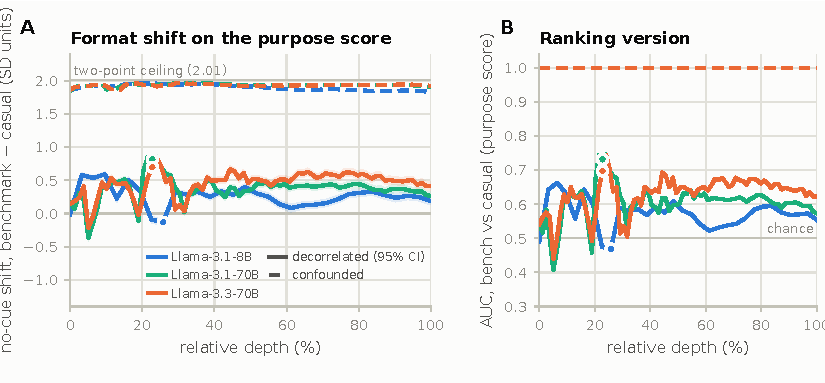
\includegraphics[width=\linewidth]{fig_results_02_nocue.pdf}
\caption{
\textbf{The format residual on no-cue items across depth.}
(A) Benchmark-minus-casual shift of the no-cue projection on the decorrelated
(solid, with 95\% payload-block bootstrap band) and confounded (dashed) purpose
scores, in units of the SD of the no-cue scores; the upper hairline is the
two-point ceiling (2.01), markers show the selected layers. The confounded
probe saturates at every depth; the decorrelated residual is small and
negative at 8B at the selected layer and positive through most of the depth
of both 70B checkpoints.
(B) The ranking version of the same quantity: AUC with which each purpose
score ranks no-cue benchmark above no-cue casual items (chance .5).
}
\label{fig:results_nocue}
\end{figure}

% ----------------------------------------------------------------------------
\subsection{Cross-format transfer and its residual}
\label{sec:results_transfer}

\citet{devbunova2026format} concluded that probes exhibit format-invariant
behavior only when format is explicitly decorrelated from context during
training. The single-format probes test this directly: a probe trained on
benchmark-format prompts only (both purposes, format constant) is evaluated on
casual-format prompts only, and conversely, with the same held-out vocabulary
folds.

\paragraph{Ranking transfers; thresholds shift.}
Without any decorrelation in training, benchmark-to-casual (B$\rightarrow$C)
and casual-to-benchmark (C$\rightarrow$B) AUC at the selected layers are
.951 / .940, .985 / .985 and .985 / .979 (Table~\ref{tab:transfer}), and both
single-format probes order every complete minimal pair correctly in every
checkpoint. A probe that has only seen one format ranks purpose in the other
nearly as well as the decorrelated probe, so the shared direction is a
property of the representation rather than of decorrelated training. Transfer
is weaker at the threshold (BA .85--.93), so ranking and decisions are
reported separately.

\paragraph{The transfer gap.}
We define the gap at each layer as decorrelated AUC minus the mean of the two
transfer AUCs (Figure~\ref{fig:results_transfer}). It is .043, .014 and .014 at
the selected layers, is smallest at intermediate depth, and widens again
toward the output (Table~\ref{tab:transfer}); integrated over normalized depth
it is .079 [.077, .082], .055 [.053, .057] and .063 [.061, .065]. A rank-64
subspace estimated from the matched format contrast inside each training fold
and projected out before the probes are refitted removes 58.5\% [57.1, 59.9],
62.8\% [61.2, 64.4] and 65.3\% [63.8, 66.9] of the integrated gap, while
changing decorrelated AUC by less than .002 on average and leaving format
decodable at AUC $\geq$ .92 (Figure~\ref{fig:results_transfer}B). The
residual is therefore largely a low-rank format-associated component of the
representation. This is a frozen-activation projection followed by probe
retraining, not a causal intervention on the model.

\begin{table}[ht]
\centering
\caption{
\textbf{Single-format probes transfer across formats, with a small
format-bound residual.}
B$\rightarrow$C: trained on benchmark-format prompts only, tested on
casual-format prompts (C$\rightarrow$B conversely), at the selected layers of
Table~\ref{tab:probe_comparison}. ``Pairs'' is the fraction of complete
minimal pairs whose evaluation member outscores its deployment twin. Gap is
decorrelated AUC minus the mean transfer AUC at the selected layer; min and
final are its trajectory minimum (with layer) and final-layer value; widening
is final minus min with a payload-block bootstrap interval.
}
\label{tab:transfer}
\footnotesize
\setlength{\tabcolsep}{3.5pt}
\begin{tabular}{lccccccc}
\toprule
Model
& \shortstack{B$\rightarrow$C\\AUC / BA}
& \shortstack{C$\rightarrow$B\\AUC / BA}
& Pairs
& \shortstack{Gap,\\selected}
& \shortstack{Gap min\\(layer)}
& \shortstack{Gap,\\final}
& \shortstack{Late widening\\{[95\% CI]}} \\
\midrule
Llama-3.1-8B  & .951 / .882 & .940 / .852 & 1.000 & .043 & .036 (14) & .095 & .059 [.052, .065] \\
Llama-3.1-70B & .985 / .926 & .985 / .921 & 1.000 & .014 & .010 (19) & .058 & .047 [.043, .052] \\
Llama-3.3-70B & .985 / .932 & .979 / .917 & 1.000 & .014 & .012 (21) & .081 & .068 [.063, .073] \\
\bottomrule
\end{tabular}
\end{table}

\begin{figure}[t]
\centering
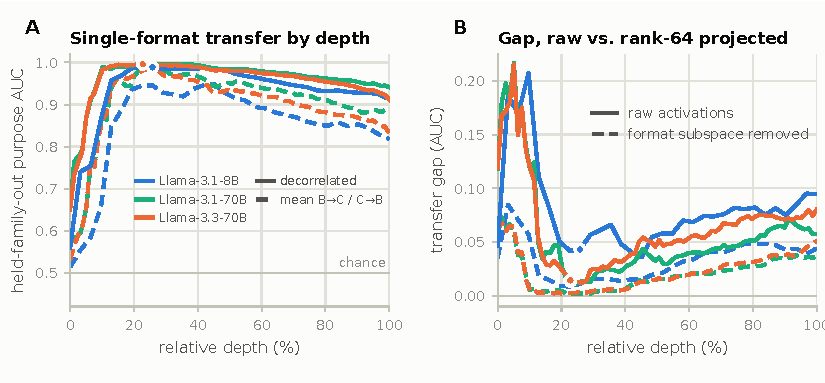
\includegraphics[width=\linewidth]{fig_results_03_transfer.pdf}
\caption{
\textbf{Cross-format transfer and the transfer gap across depth.}
(A) Decorrelated purpose AUC (solid) and the mean of the two single-format
transfer AUCs (dashed) across relative depth; markers show the selected
layers. (B) The transfer gap (decorrelated minus mean transfer AUC) on the raw
activations (solid) and after projecting out the cross-fitted rank-64
matched-format subspace and refitting the probes (dashed). The gap is
smallest at intermediate depth, widens toward the output, and is more than
half removed by the projection at every depth where purpose is formed.
}
\label{fig:results_transfer}
\end{figure}

\paragraph{Controls.}
Holding the number of training payload blocks fixed at Llama-3.1-8B layer 12,
equal-size mixed training gives AUC .980 against .959 and .954 for
benchmark-only and casual-only training, so the transfer penalty is not a
row-count artifact (Table~\ref{tab:equaln}). With the purpose statement
excised, the evaluation and deployment renderings are byte-identical and
text-only probes score .500 by construction; with it present, word-level
probes under the same held-vocabulary folds stay at chance while character
n-grams reach .71 on the cue sentence alone, far below the activation probes'
.99 (Table~\ref{tab:text_controls}). In an earlier single-template pilot on a
separate 80-block freeze, single-format transfer AUC was only .78--.96, with
balanced accuracy collapsing to .50--.58 in three of six cells
(Table~\ref{tab:pilot}), so the invariance reported here is across a family
of wrappers rather than between two fixed templates.

% ============================================================================
% APPENDIX MATERIAL moved out of Section 3.3 (control tables referenced by the
% "Controls" paragraph). Delete this block if the tables are not wanted, and
% drop the three \ref{tab:...} pointers above.
% ============================================================================
\appendix
\section{Control tables for Section~\ref{sec:results_transfer}}
\label{app:controls}

\begin{table}[ht]
\centering
\caption{
\textbf{Equal-training-size control, Llama-3.1-8B, layer 12.}
Each regime trains on the same number of payload blocks per held-out family
(one format per block); the mixed regime balances format over blocks. Values
are means over four fixed assignment seeds; intervals are means of the
1,000-replicate payload-block bootstrap limits. Development control for one
checkpoint and one predeclared layer. An exact-row version on all three
checkpoints (identical blocks, pair units and rows per regime; eight seeds;
one fixed depth) gives a mixed-minus-best-specialist AUC contrast of $+.009$
[$+.008$, $+.010$] with the logistic probe and $-.004$ [$-.005$, $-.003$] with a
diagonal-LDA probe, so the sign of the small mixed-training advantage is
estimator-dependent.
}
\label{tab:equaln}
\small
\setlength{\tabcolsep}{6pt}
\begin{tabular}{lcc}
\toprule
Training regime & AUC [95\% CI] & BA [95\% CI] \\
\midrule
Benchmark-only    & .959 [.955, .963] & .895 [.889, .901] \\
Casual-only       & .954 [.950, .958] & .878 [.871, .884] \\
Equal-size mixed  & .980 [.977, .982] & .924 [.918, .930] \\
\bottomrule
\end{tabular}
\end{table}

\begin{table}[ht]
\centering
\caption{
\textbf{Text-only probes for purpose under held-out splits.}
TF--IDF logistic regression on the rendered text; held-family splits are the
five leave-one-purpose-vocabulary-family-out folds used for the activation
probes. Cue-excised rows remove the purpose statement by its recorded span,
after which the eval/deploy twins are byte-identical. Cue-present rows give the
mean held-family AUC with the maximum single-fold AUC in parentheses
(word unigrams; character 3--5-grams; the cue-excised battery uses word
1--2-grams and character 2--5-grams). Nuisance
probes (format .798, template identity .908 vs.\ chance .077, response
contract .983 vs.\ chance .200) are reported, not gated. Cue-present rows are a
development-only audit on the full320 stated stratum (7,680 rows).
}
\label{tab:text_controls}
\small
\setlength{\tabcolsep}{5pt}
\begin{tabular}{llcc}
\toprule
Condition & Text scope & Word n-gram AUC & Char n-gram AUC \\
\midrule
Cue excised, held template                 & full prompt          & .500 & .500 \\
Cue excised, held template $\times$ family & full prompt          & .500 & .500 \\
Cue present, held family                   & cue sentence only    & .498 (.500) & .709 (.881) \\
Cue present, held family                   & full prompt          & .535 (.583) & .629 (.752) \\
Cue present, held family                   & scaffold without cue & .500 (.500) & .500 (.500) \\
\bottomrule
\end{tabular}
\end{table}

\begin{table}[ht]
\centering
\caption{
\textbf{Preliminary single-template pilot (separate 80-block freeze).}
One benchmark and one casual template per purpose, same vocabulary folds and
probe recipe; values at each checkpoint's decorrelated-AUC peak layer. Not
pooled with the main results.
}
\label{tab:pilot}
\small
\setlength{\tabcolsep}{5pt}
\begin{tabular}{lcccc}
\toprule
Model & Layer & \shortstack{Decorrelated\\AUC / BA} & \shortstack{B$\rightarrow$C\\AUC / BA} & \shortstack{C$\rightarrow$B\\AUC / BA} \\
\midrule
Llama-3.1-8B  & 12 & .992 / .958 & .782 / .715 & .786 / .575 \\
Llama-3.1-70B & 31 & .998 / .977 & .871 / .523 & .957 / .504 \\
Llama-3.3-70B & 17 & .995 / .962 & .955 / .823 & .822 / .694 \\
\bottomrule
\end{tabular}
\end{table}
